% Options for packages loaded elsewhere
% Options for packages loaded elsewhere
\PassOptionsToPackage{unicode}{hyperref}
\PassOptionsToPackage{hyphens}{url}
\PassOptionsToPackage{dvipsnames,svgnames,x11names}{xcolor}
%
\documentclass[
]{agujournal2019}
\usepackage{xcolor}
\usepackage{amsmath,amssymb}
\setcounter{secnumdepth}{5}
\usepackage{iftex}
\ifPDFTeX
  \usepackage[T1]{fontenc}
  \usepackage[utf8]{inputenc}
  \usepackage{textcomp} % provide euro and other symbols
\else % if luatex or xetex
  \usepackage{unicode-math} % this also loads fontspec
  \defaultfontfeatures{Scale=MatchLowercase}
  \defaultfontfeatures[\rmfamily]{Ligatures=TeX,Scale=1}
\fi
\usepackage{lmodern}
\ifPDFTeX\else
  % xetex/luatex font selection
\fi
% Use upquote if available, for straight quotes in verbatim environments
\IfFileExists{upquote.sty}{\usepackage{upquote}}{}
\IfFileExists{microtype.sty}{% use microtype if available
  \usepackage[]{microtype}
  \UseMicrotypeSet[protrusion]{basicmath} % disable protrusion for tt fonts
}{}
\makeatletter
\@ifundefined{KOMAClassName}{% if non-KOMA class
  \IfFileExists{parskip.sty}{%
    \usepackage{parskip}
  }{% else
    \setlength{\parindent}{0pt}
    \setlength{\parskip}{6pt plus 2pt minus 1pt}}
}{% if KOMA class
  \KOMAoptions{parskip=half}}
\makeatother
% Make \paragraph and \subparagraph free-standing
\makeatletter
\ifx\paragraph\undefined\else
  \let\oldparagraph\paragraph
  \renewcommand{\paragraph}{
    \@ifstar
      \xxxParagraphStar
      \xxxParagraphNoStar
  }
  \newcommand{\xxxParagraphStar}[1]{\oldparagraph*{#1}\mbox{}}
  \newcommand{\xxxParagraphNoStar}[1]{\oldparagraph{#1}\mbox{}}
\fi
\ifx\subparagraph\undefined\else
  \let\oldsubparagraph\subparagraph
  \renewcommand{\subparagraph}{
    \@ifstar
      \xxxSubParagraphStar
      \xxxSubParagraphNoStar
  }
  \newcommand{\xxxSubParagraphStar}[1]{\oldsubparagraph*{#1}\mbox{}}
  \newcommand{\xxxSubParagraphNoStar}[1]{\oldsubparagraph{#1}\mbox{}}
\fi
\makeatother


\usepackage{longtable,booktabs,array}
\usepackage{calc} % for calculating minipage widths
% Correct order of tables after \paragraph or \subparagraph
\usepackage{etoolbox}
\makeatletter
\patchcmd\longtable{\par}{\if@noskipsec\mbox{}\fi\par}{}{}
\makeatother
% Allow footnotes in longtable head/foot
\IfFileExists{footnotehyper.sty}{\usepackage{footnotehyper}}{\usepackage{footnote}}
\makesavenoteenv{longtable}
\usepackage{graphicx}
\makeatletter
\newsavebox\pandoc@box
\newcommand*\pandocbounded[1]{% scales image to fit in text height/width
  \sbox\pandoc@box{#1}%
  \Gscale@div\@tempa{\textheight}{\dimexpr\ht\pandoc@box+\dp\pandoc@box\relax}%
  \Gscale@div\@tempb{\linewidth}{\wd\pandoc@box}%
  \ifdim\@tempb\p@<\@tempa\p@\let\@tempa\@tempb\fi% select the smaller of both
  \ifdim\@tempa\p@<\p@\scalebox{\@tempa}{\usebox\pandoc@box}%
  \else\usebox{\pandoc@box}%
  \fi%
}
% Set default figure placement to htbp
\def\fps@figure{htbp}
\makeatother


% definitions for citeproc citations
\NewDocumentCommand\citeproctext{}{}
\NewDocumentCommand\citeproc{mm}{%
  \begingroup\def\citeproctext{#2}\cite{#1}\endgroup}
\makeatletter
 % allow citations to break across lines
 \let\@cite@ofmt\@firstofone
 % avoid brackets around text for \cite:
 \def\@biblabel#1{}
 \def\@cite#1#2{{#1\if@tempswa , #2\fi}}
\makeatother
\newlength{\cslhangindent}
\setlength{\cslhangindent}{1.5em}
\newlength{\csllabelwidth}
\setlength{\csllabelwidth}{3em}
\newenvironment{CSLReferences}[2] % #1 hanging-indent, #2 entry-spacing
 {\begin{list}{}{%
  \setlength{\itemindent}{0pt}
  \setlength{\leftmargin}{0pt}
  \setlength{\parsep}{0pt}
  % turn on hanging indent if param 1 is 1
  \ifodd #1
   \setlength{\leftmargin}{\cslhangindent}
   \setlength{\itemindent}{-1\cslhangindent}
  \fi
  % set entry spacing
  \setlength{\itemsep}{#2\baselineskip}}}
 {\end{list}}
\usepackage{calc}
\newcommand{\CSLBlock}[1]{\hfill\break\parbox[t]{\linewidth}{\strut\ignorespaces#1\strut}}
\newcommand{\CSLLeftMargin}[1]{\parbox[t]{\csllabelwidth}{\strut#1\strut}}
\newcommand{\CSLRightInline}[1]{\parbox[t]{\linewidth - \csllabelwidth}{\strut#1\strut}}
\newcommand{\CSLIndent}[1]{\hspace{\cslhangindent}#1}



\setlength{\emergencystretch}{3em} % prevent overfull lines

\providecommand{\tightlist}{%
  \setlength{\itemsep}{0pt}\setlength{\parskip}{0pt}}



 


\usepackage{url} %this package should fix any errors with URLs in refs.
\usepackage{lineno}
\usepackage[inline]{trackchanges} %for better track changes. finalnew option will compile document with changes incorporated.
\usepackage{soul}
\linenumbers
\makeatletter
\@ifpackageloaded{caption}{}{\usepackage{caption}}
\AtBeginDocument{%
\ifdefined\contentsname
  \renewcommand*\contentsname{Table of contents}
\else
  \newcommand\contentsname{Table of contents}
\fi
\ifdefined\listfigurename
  \renewcommand*\listfigurename{List of Figures}
\else
  \newcommand\listfigurename{List of Figures}
\fi
\ifdefined\listtablename
  \renewcommand*\listtablename{List of Tables}
\else
  \newcommand\listtablename{List of Tables}
\fi
\ifdefined\figurename
  \renewcommand*\figurename{Figure}
\else
  \newcommand\figurename{Figure}
\fi
\ifdefined\tablename
  \renewcommand*\tablename{Table}
\else
  \newcommand\tablename{Table}
\fi
}
\@ifpackageloaded{float}{}{\usepackage{float}}
\floatstyle{ruled}
\@ifundefined{c@chapter}{\newfloat{codelisting}{h}{lop}}{\newfloat{codelisting}{h}{lop}[chapter]}
\floatname{codelisting}{Listing}
\newcommand*\listoflistings{\listof{codelisting}{List of Listings}}
\makeatother
\makeatletter
\makeatother
\makeatletter
\@ifpackageloaded{caption}{}{\usepackage{caption}}
\@ifpackageloaded{subcaption}{}{\usepackage{subcaption}}
\makeatother
\usepackage{bookmark}
\IfFileExists{xurl.sty}{\usepackage{xurl}}{} % add URL line breaks if available
\urlstyle{same}
\hypersetup{
  pdftitle={La Palma Earthquake Mechanisms},
  pdfauthor={Travis Zalesky},
  pdfkeywords={ephemeral (transient)
water, flood, LandSat, MODIS, playa, remote sensing, satellite
data, sheet flow, synthetic aperture radar (SAR)},
  colorlinks=true,
  linkcolor={blue},
  filecolor={Maroon},
  citecolor={Blue},
  urlcolor={Blue},
  pdfcreator={LaTeX via pandoc}}



\draftfalse

\begin{document}
\title{La Palma Earthquake Mechanisms}

\authors{Travis Zalesky\affil{1}}
\affiliation{1}{University of Arizona, }
\correspondingauthor{Travis Zalesky}{travisz@arizona.edu}


\begin{abstract}
A variety of remote sensing methods are investigated for their ability
to detect ephemeral water bodies across the state of Arizona. The
strengths and weaknesses of each are discussed.
\end{abstract}

\section*{Plain Language Summary}
Results and methods for detecting transient water bodies using satellite
data.




\section{Introduction}\label{introduction}

As part of the Arizona Tri-University Recharge (ATUR) project, multiple
methods for identifying and quantifying ephemeral water bodies across
the state of Arizona (AZ) are investigated. For reasons that will be
discussed, accurate identification of ephemeral, or temporary, water
bodies is a challenge, and efforts to-date have shown limited success.
Methods, results, and challenges are discussed, and potential paths
forward are explored.

Ephemeral water bodies are common features in the arid American
southwest. Typically very shallow, these water bodies range in size from
a few cm rock pools to flash flood associated sheet flow, and playas up
to several km in diameter (Crawford, 1981; Whitford \& Duval, 2020).
While playas and intermittent streams are well mapped across AZ, there
is no consensus on the volume of water which flows through these
systems. More to the point, there is no widely accepted estimate of the
volume of water which either evaporates or recharges from these
internally draining basins.

It is not clear what fraction of water which flows onto a playa is
evaporated vs.~recharged. On the one hand, the nature of playas results
in the slow accumulation of surface salts and fine sediments (clays and
silts), which are generally impervious and detrimental to infiltration
and subsequent recharge (Whitford \& Duval, 2020). Additionally, playas
may be an oasis for drought resistant flora, increasing local
evapotranspiration, even after shallow surface soil layers have dried
out (Crawford, 1981). Alternately, these mineral rich surface crusts may
be prone to expansion when wetted, and are frequently characterized by
deep cracks which provide avenues for water infiltration below the
impervious layers (Whitford \& Duval, 2020). While the majority of water
flowing onto most playas will be lost to evaporation, there may be
specific playas where water loss by infiltration may exceed evaporation
(Whitford \& Duval, 2020). At least initially, we will assume that all
water flowing onto playas shall be evaporated, subject to later
reevaluation and refinement.

The primary target of this study is to estimate and quantify the volume
of water flowing into small to medium sized playas, on the order of
\textasciitilde50 m to \textasciitilde1 km in diameter, although
identification of sheet flow may also be incidental. The general method
outlined is to use remote sensing technology to identify standing water
broadly across the study area, across a time series. By identifying
standing water, and assuming a constant water depth, water volume can be
estimated. Additionally, an approximation of ``continuously wetted''
days can provide an initial estimate of evaporation rates, and through
comparison with alternate evapotranspiration estimates, may be useful
for estimating infiltration rate (e.g.~if water loss rate is 2
cm\^{}3/day and the evapotranspiration rate is 1.5 cm\^{}3/day then the
implied infiltration rate would be 0.5 cm\^{}3/day).

The study area used for method development is primarily Hualapai Playa
(a.k.a. Red Lake), located in northwest AZ, approx. 60 km
south-southwest of Lake Mead (Figure~\ref{fig-PlayaRef}). This ephemeral
playa is roughly 1 km in diameter, and is one of the largest playas in
AZ. Furthermore, local landowners surrounding Hualapai Playa have
expressed sincere interest in our project, creating additional
public-relations incentives related to this particular playa. Lastly,
it's proximity to Lake Mead and Lake Mohave provide a convenient region
for testing these methods against known areas of permanent surface
water.

\begin{figure}

\centering{

\pandocbounded{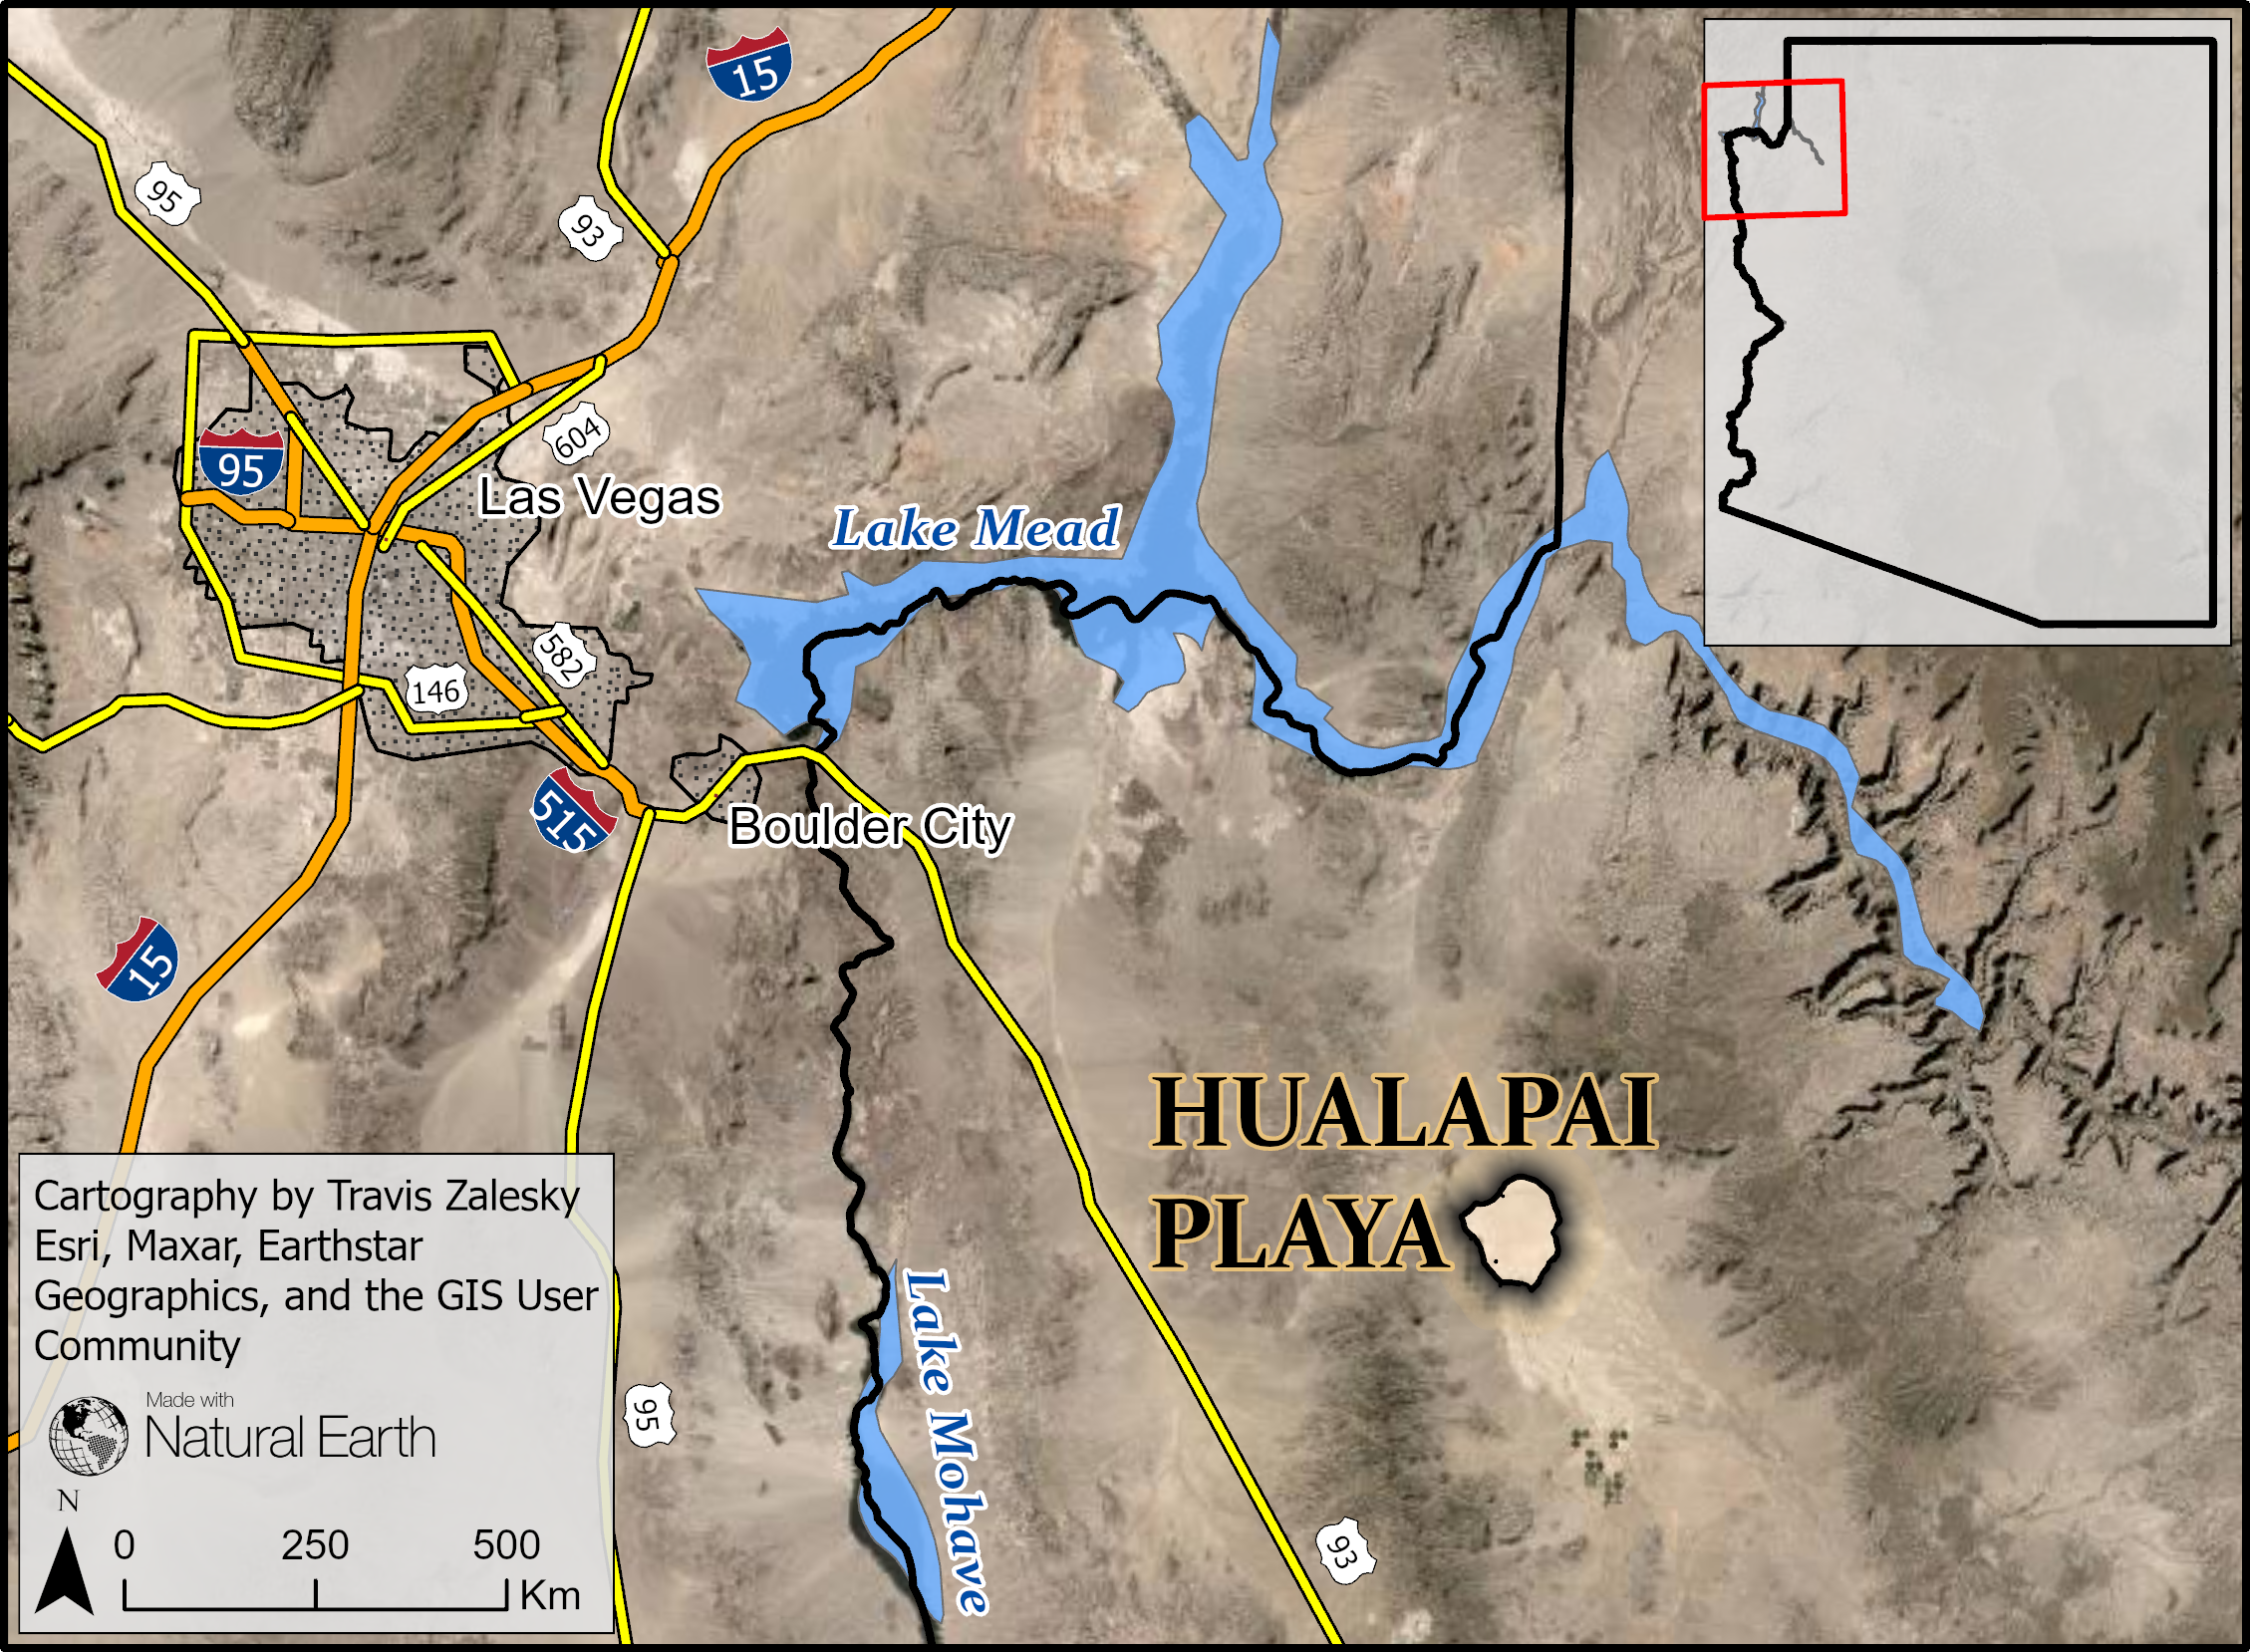
\includegraphics[keepaspectratio]{images/Hualapai_Playa_Reference.png}}

}

\caption{\label{fig-PlayaRef}Hualapai Playa locator map.}

\end{figure}%

One of the most challenging aspects of developing these methods is the
lack of quality ground-truth data. Without existing data regarding date
and duration of standing water within these ephemeral features, it is
extremely difficult to validate our methods. While reasonable
assumptions can be made about method accuracy (or inaccuracy as the case
may be), any method, either those presented herein, or future methods
not yet considered, will have to be validated using a known and well
characterized ephemeral water body, ideally within AZ, or elsewhere in a
similar arid environment.

\section{Methods \& Results}\label{methods-results}

\section{Further Recommendations}\label{further-recommendations}

\section{Conclusion}\label{conclusion}

\section*{References}\label{references}
\addcontentsline{toc}{section}{References}

\phantomsection\label{refs}
\begin{CSLReferences}{1}{0}
\vspace{1em}

\bibitem[\citeproctext]{ref-Clifford_Crawford}
Crawford, C. S. (1981). Chapter 17 - the invertebrate community of
ephemeral waters. In \emph{Biology of desert invertebrates} (pp.
234--247). Springer-Verlag.

\bibitem[\citeproctext]{ref-Whitford_Duval_2020}
Whitford, W. G., \& Duval, B. D. (2020). \emph{Chapter 8 - consumers and
their effects} (W. G. Whitford \& B. D. Duval, Eds.; pp. 203--263).
Academic Press. \url{https://doi.org/10.1016/B978-0-12-815055-9.00008-4}

\end{CSLReferences}




\end{document}
